\documentclass[11pt]{article} 

\usepackage[margin=1.5in]{geometry}
\usepackage{multicol}
\usepackage{lmodern}
\usepackage{microtype}
\usepackage{booktabs}

\usepackage{amsmath}
\usepackage{amssymb}
\usepackage{sectsty}
\allsectionsfont{\normalfont\sffamily\bfseries}

\usepackage{siunitx}
\usepackage[font=sf]{caption}
\usepackage[font=sf]{floatrow}
\usepackage{titlesec}
\usepackage{lipsum}
\usepackage{etoolbox}
\usepackage{graphicx}
\usepackage{enumitem}
\usepackage{wrapfig}
\usepackage{listings}
%\usepackage{hyperref}
\usepackage{fancyhdr}
\usepackage{tikz}
\usetikzlibrary{calc}
\usepackage{pgfplots}
\usepackage{defs}

\lstset{
basicstyle=\small\ttfamily,
columns=flexible,
breaklines=true
}

\pagestyle{fancy}
\rhead{\sffamily Lasanga Controller User Guide}
\lhead{\sffamily SSI Balloons}
%\rhead{\sffamily John Dean}
\rfoot{\footnotesize \sffamily \today}
%\setlength\parindent{0in}
\usepackage[utf8]{inputenc}

\def\sc{\begin{quote}\begin{lstlisting}}
\def\ec{\end{lstlisting}\end{quote}}
\def\tt#1{{\ttfamily #1}}
\linespread{1}
\begin{document}

\section{Overview}

Lasanga consists of two nested feedback loops, an outer loop that tracks an altitude and commands a velocity, and an inner loop that tracks a velocity and commands a change in lift. A block diagram of the idealized system is shown below\footnote{For those without much control background: block diagrams represents the structure of a control system. Each block represents some kind of system with inputs and outputs. Each solid line with an arrow on it represent a value and show how outputs of some blocks are connected to inputs of others. Circles represent adding or subtracting, (the +/- sign where the arrow enters the circle indicates which) while blocks represent \emph{transfer functions}. Transfer functions are linear systems represented in the Leplace domain. Without going into too much detail, a simple Transfer function $K(s) = 5$ ($s$ is the variable in the Laplace domain) is simply scalar multiplication by 5. $K(s) = 1/s$ represents integration of a value, and $K(s) = s$ represents the derivative of a value.}

\begin{figure}[h!]
\caption{Idealized system block diagram}
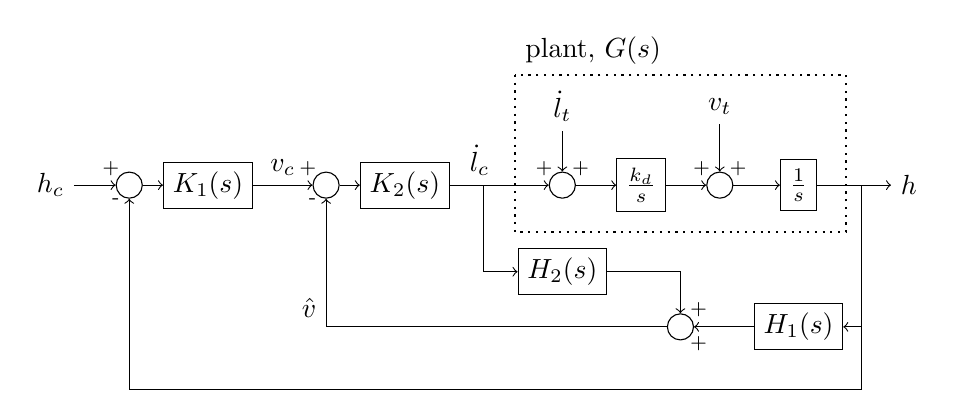
\begin{tikzpicture}[scale=2,
     block/.style = {draw, rectangle,node distance=1cm},
     input/.style = {node distance=1cm},
     output/.style = {node distance=1cm},
     arrow/.style={draw, -latex,node distance=2cm},
     pinstyle/.style = {pin edge={latex-, black,node distance=2cm}},
     sum/.style = {draw, circle, node distance=1cm},
     gain/.style = {regular polygon, regular polygon sides=3,draw, fill=white, text width=1em,
      inner sep=0mm, outer sep=0mm,
      shape border rotate=-90}
    ]
        
    \node [input] (hcmd) {$h_c$};
    \node [sum,right of=hcmd] (hsum) {};    
    \node [block,right of=hsum, node distance=1cm] (K1) {$K_1(s)$};
    \node [sum,right of=K1, node distance=1.5cm] (vsum) {};
    \node [block, right of=vsum] (K2) {$K_2(s)$};
    \node [sum, right of=K2, node distance=2cm] (dlift) {};
    \node [input, above of=dlift] (ldist) {$\dot l_t$};
    \node [block, right of=dlift] (lint) {$\frac{k_d}{s}$};
    \node [sum, right of=lint] (velocity) {};
    \node [input, above of=velocity] (vdist) {$v_t$};
    \node [block, right of=velocity] (vint) {$\frac{1}{s}$};
    \node [output, right of=vint,node distance=1.4cm] (h) {$h$};
    \node [block, below of=vint,node distance=1.8cm] (H1) {$H_1(s)$};
    \node [block, below of=dlift,node distance=1.1cm] (H2) {$H_2(s)$};
    \node [sum, left of=H1,node distance=1.5cm] (fsum) {};

    \draw[->] (hcmd) -- (hsum) node [above left] {\scriptsize +};
    \draw[->] (hsum) -- (K1);
    \draw[->] (K1) -- node [above] {$v_c$} (vsum) node [above left] {\scriptsize +};
    \draw[->] (vsum) -- (K2);
    \draw[->] (K2) -- node [above left] {$\dot l_c$} (dlift)  node [above left] {\scriptsize +};
    \draw[->] (ldist) -- (dlift) node [above right] {\scriptsize +};
    \draw[->] (dlift) -- (lint);
    \draw[->] (lint) -- (velocity) node [above left] {\scriptsize +};
    \draw[->] (vdist) -- (velocity) node [above right] {\scriptsize +};
    \draw[->] (velocity) -- (vint) node [above right] {};
    \draw[->] (vint) -- (h) node [above right] {};
    \draw  (h) ++ (-.3,0) -- ++(0,-1.3) coordinate (fb);
    \draw[->]  (h) ++ (-.3,0) |- (H1);
    \draw[->] (K2) ++ (0.5,0) |- (H2);
    \draw[->] (H1) -- (fsum) node [below right] {\scriptsize +};
    \draw[->] (H2) -| (fsum) node [above right] {\scriptsize +}; 
    \draw[->] (fsum) -| node [above left] {$\hat v$} (vsum) node [below left] {\scriptsize -};
    \draw[->] (fb) -| (hsum) node [below left] {\scriptsize -};
    \draw[thick,dotted] ($(dlift)+(-.3cm,.7cm)$) node [above right] {plant, $G(s)$} rectangle ($(vint)+(.3cm,-.3cm)$) ;

\end{tikzpicture}\\
\vspace{0.5cm}
\begin{tabular}{r l}
$K_1(s) = K_h$ & proportional altitude loop compensator \\
$K_2(s) = K_v$ & proportional velocity loop compensator \\ 
$H_1(s)$ & veloctiy estimator, lowpass filter on derivative of position\\
$H_2(s)$ & integration with decay \footnotesize (estimate of effect of actions, decays to 0 over time) \vspace{.3cm}\\
$h_c$ & commanded altitude \footnotesize (set by Flight Controller) \\
$v_c$ & commanded velocity \footnotesize (output of position loop) \\
$\dot l_c$ & commanded change in lift per unit time  \footnotesize (output of velocity loop)\\
$\dot l_t$ & atmospheric disturbances that change balloon lift  \footnotesize (heating/cooling)\\
$v_t$ & atmospheric disturbances that change balloon velocity \footnotesize (turbulence)\\
$\hat v$ & estimate of velocity\\
$h$ & actual balloon altitude\\

\end{tabular}
\end{figure}

``Plant'' or $G(s)$ refers to the \emph{system} (atmosphere + balloon) dynamics, whereas everything else represents the control feedback structure that is computed in the ValBal flight code.

\section{Constants Definitions}
\begin{table}[h!]
\rmfamily
\begin{tabular}{l r  l} 
\sffamily \textbf{Contstant} &\sffamily \textbf{Default} &\sffamily \textbf{Description} \\

{\ttfamily freq}              & 20 & frequency that the controller is called at (Hz) \\
{\ttfamily k\_v            }  & 1e-3  & velocity Gain \\
{\ttfamily k\_h            }  & 1.5e-3  & altitude Gain   \\
{\ttfamily b\_dldt         }  & 6e-4  & lift rate of ballast actions (kg/s) \\
{\ttfamily v\_dldt         }  & 3e-3  & lift rate of valve actions  (kg/s) \\
{\ttfamily b\_tmin         }  & 5  & minimum ballast interval (s)   \\
{\ttfamily v\_tmin         }  & 5  & minimum valve interval (s)\\
{\ttfamily h\_cmd          }  & 13000  & commanded altitude (m)   \\
{\ttfamily kfuse           }  & 7  & atmosphere gain for velocity estimator   \\
{\ttfamily kfuse\_val      }  & 0.5  & velocity estimator gain modifier for valve  \\
{\ttfamily ss\_error\_thresh} & 750  & error tollerance for deadband (m) \\
\end{tabular}
\end{table}

\end{document}

